\documentclass[12pt,a4paper]{article}
\usepackage[utf8]{inputenc}
\usepackage[T1]{fontenc}
\usepackage[provide=*,french]{babel}
\usepackage{lmodern}
\usepackage{geometry}
\geometry{margin=2.5cm}
\usepackage{amsmath,amssymb}
\usepackage{graphicx}
\usepackage{booktabs}
\usepackage{array}
\usepackage{float}
\usepackage{xcolor}
\usepackage{listings}
\usepackage{hyperref}
\usepackage{fancyhdr}
\usepackage{microtype}
\usepackage{enumitem}
\definecolor{bleu}{HTML}{145DA0}
\definecolor{vert}{HTML}{2A9D8F}
\hypersetup{colorlinks=true,linkcolor=bleu,citecolor=vert,urlcolor=bleu,
  pdftitle={Implémentation de l'algorithme des nuées dynamiques},
  pdfauthor={KABONGO TSHIATA ETIENNE}}
\pagestyle{fancy}
\fancyhf{}
\lhead{Science des données -- M1 IA}
\rhead{Nuées dynamiques}
\cfoot{\thepage}
\setlength{\headheight}{15pt}
\setlength{\parindent}{0pt}
\setlength{\parskip}{0.55em}
\lstset{language=Python,basicstyle=\ttfamily\small,keywordstyle=\color{bleu}\bfseries,
  commentstyle=\color{vert},stringstyle=\color{orange!60!black},frame=single,
  breaklines=true,showstringspaces=false,numbers=left,numberstyle=\tiny,
  xleftmargin=1.5em,framexleftmargin=1em}

\begin{document}
\begin{titlepage}
  \centering
  {\large UNIVERSITÉ DE KINSHASA\par}
  \vspace{0.4cm}
  {\large Master 1 -- Intelligence Artificielle\par}
  \vfill
  {\color{bleu}\rule{\textwidth}{1.4pt}\par}
  \vspace{0.5cm}
  {\Huge\bfseries Implémentation de l'algorithme des nuées dynamiques\par}
  \vspace{0.35cm}
  {\LARGE From scratch en Python\par}
  \vspace{0.5cm}
  {\color{bleu}\rule{\textwidth}{1.4pt}\par}
  \vfill
  \begin{tabular}{>{\bfseries}p{4.2cm}p{8cm}}
    Étudiant : & KABONGO TSHIATA ETIENNE\\
    Niveau : & M1 IA\\
    Cours : & Science des données\\
    Sujet : & Implémentation de l'algorithme des nuées dynamiques (from scratch)\\
    Année académique : & 2025--2026
  \end{tabular}
  \vfill
  {\large Kinshasa, septembre 2026\par}
\end{titlepage}

\tableofcontents
\newpage

\section{Introduction}
L'apprentissage non supervisé cherche à extraire une structure à partir de
données qui ne possèdent pas d'étiquette connue. Parmi ses tâches centrales,
la classification automatique (\emph{clustering}) consiste à constituer des
groupes homogènes : les observations d'un même groupe doivent être proches,
tandis que celles de groupes différents doivent être éloignées.

L'algorithme des nuées dynamiques, étroitement lié à la méthode des
$k$-moyennes, alterne une phase d'affectation aux centres les plus proches et
une phase de représentation de chaque classe par son centre de gravité. Cette
famille de méthodes trouve notamment ses racines dans les travaux de
MacQueen~\cite{macqueen1967} et de Lloyd~\cite{lloyd1982}.

Ce travail présente les fondements mathématiques, une implémentation personnelle
en Python et une expérimentation reproductible. L'objectif n'est pas d'appeler
une fonction prête à l'emploi : le calcul des distances, les affectations, les
centres, l'inertie et les critères d'arrêt sont programmés directement.

\section{Problématique et objectifs}
Soit une matrice de données $X\in\mathbb{R}^{n\times p}$. Comment partitionner
ses $n$ observations en $k$ classes compactes sans disposer d'étiquettes ?
L'enjeu est de construire une procédure compréhensible, correcte et robuste aux
aléas de l'initialisation.

Les objectifs spécifiques sont :
\begin{itemize}[itemsep=2pt]
  \item formaliser le problème d'optimisation et les étapes de l'algorithme ;
  \item coder toutes les opérations fondamentales sans KMeans externe ;
  \item gérer les classes vides et les initialisations défavorables ;
  \item observer la convergence et apprécier le choix de $k$ ;
  \item vérifier séparément la cohérence des résultats avec une référence.
\end{itemize}

\section{Fondements théoriques}
\subsection{Partition et centre de gravité}
Une partition $P=(C_1,\ldots,C_k)$ divise l'ensemble des observations en
classes disjointes. Pour une classe non vide $C_j$, son centre de gravité est
la moyenne de ses observations :
\begin{equation}
  \boldsymbol{\mu}_j=\frac{1}{|C_j|}\sum_{\mathbf{x}_i\in C_j}\mathbf{x}_i.
\end{equation}
Ce centre minimise la somme des distances euclidiennes au carré aux membres de
la classe~\cite{hastie2009}.

\subsection{Distance et fonction objectif}
La distance euclidienne entre une observation $\mathbf{x}_i$ et un centre
$\boldsymbol{\mu}_j$ est
\begin{equation}
 d(\mathbf{x}_i,\boldsymbol{\mu}_j)=
 \sqrt{\sum_{r=1}^{p}(x_{ir}-\mu_{jr})^2}.
\end{equation}
Comme la racine carrée est croissante, l'affectation peut employer directement
la distance au carré. L'inertie intra-classe à minimiser vaut
\begin{equation}\label{eq:objectif}
 J(P,\boldsymbol{\mu})=\sum_{j=1}^{k}\sum_{\mathbf{x}_i\in C_j}
 \left\|\mathbf{x}_i-\boldsymbol{\mu}_j\right\|_2^2.
\end{equation}

\subsection{Alternance des deux phases}
À centres fixés, chaque observation rejoint la classe de son centre le plus
proche :
\begin{equation}\label{eq:affectation}
 z_i=\underset{1\leq j\leq k}{\arg\min}\;
 \|\mathbf{x}_i-\boldsymbol{\mu}_j\|_2^2.
\end{equation}
À partition fixée, les centres sont recalculés par
\begin{equation}\label{eq:maj}
 \boldsymbol{\mu}_j^{(t+1)}=\frac{1}{|C_j^{(t)}|}
 \sum_{\mathbf{x}_i\in C_j^{(t)}}\mathbf{x}_i.
\end{equation}
Chacune de ces phases ne peut augmenter l'objectif~\eqref{eq:objectif}. Comme
il existe un nombre fini de partitions, la procédure atteint un point fixe en
un nombre fini d'étapes. Ce point est toutefois un optimum local, pas
nécessairement l'optimum global.

\section{Algorithme proposé}
\subsection{Pseudo-code}
\begin{enumerate}
  \item choisir $k$ observations distinctes comme centres initiaux ;
  \item calculer toutes les distances au carré ;
  \item affecter chaque observation au centre le plus proche ;
  \item remplacer chaque centre par la moyenne de sa classe ;
  \item si une classe est vide, replacer son centre sur une observation mal
        représentée ;
  \item calculer l'inertie et mémoriser sa valeur ;
  \item arrêter si le déplacement global des centres est inférieur à
        $\varepsilon$, si la partition est stable, ou si la limite d'itérations
        est atteinte ; sinon retourner à l'étape 2 ;
  \item répéter l'ensemble avec plusieurs initialisations et conserver la
        solution de plus faible inertie.
\end{enumerate}

\subsection{Critères d'arrêt et complexité}
Le déplacement est mesuré par la norme de Frobenius :
\begin{equation}
 \Delta^{(t)}=\|M^{(t+1)}-M^{(t)}\|_F.
\end{equation}
L'arrêt intervient lorsque $\Delta^{(t)}\leq\varepsilon$ ou lorsque deux
partitions successives sont identiques. Pour $T$ itérations, le coût dominant
du calcul des distances est $O(Tnkp)$ et le stockage de la matrice des
distances demande $O(nk)$.

\subsection{Choix de conception}
L'implémentation utilise une graine pseudo-aléatoire pour assurer la
reproductibilité. Plusieurs démarrages réduisent le risque d'un mauvais optimum
local. En cas de classe vide, le nouveau centre est choisi parmi les points qui
contribuent le plus à l'inertie courante. Une méthode \texttt{predict} permet
enfin d'affecter de nouvelles observations aux centres appris.

\section{Implémentation from scratch}
Le cœur du calcul des distances est le suivant :
\begin{lstlisting}
def _distances_carre(X, centres):
    differences = X[:, np.newaxis, :] - centres[np.newaxis, :, :]
    return np.sum(differences * differences, axis=2)
\end{lstlisting}
L'affectation et l'inertie ne nécessitent ensuite que l'indice du minimum de
chaque ligne et la somme des distances retenues :
\begin{lstlisting}
distances = self._distances_carre(X, centres)
etiquettes = np.argmin(distances, axis=1)
inertie = np.sum(distances[np.arange(X.shape[0]), etiquettes])
\end{lstlisting}
NumPy sert ici uniquement à représenter les tableaux et à effectuer les
opérations arithmétiques. La logique de clustering est entièrement contenue
dans la classe \texttt{NueesDynamiques}. Le fichier complet est fourni dans
\texttt{src/nuees\_dynamiques.py}.

\section{Protocole expérimental}
\subsection{Jeu de données}
Le jeu synthétique contient 450 observations bidimensionnelles, réparties en
trois nuages gaussiens de 150 points. Leurs moyennes génératrices sont
$(-3,-2)$, $(0{,}2,3{,}2)$ et $(3{,}6,-0{,}8)$, avec des dispersions différentes.
Une graine fixée à 42 permet de régénérer exactement les mêmes données. Le CSV
produit est inclus dans le projet.

\subsection{Paramètres}
L'expérience principale emploie $k=3$, au maximum 200 itérations, une tolérance
de $10^{-6}$ et 20 initialisations. L'étude du coude compare ensuite les valeurs
$k=1,\ldots,8$ avec 15 initialisations pour chacune.

\section{Résultats et analyse}
\subsection{Partition obtenue}
\begin{figure}[H]
 \centering
 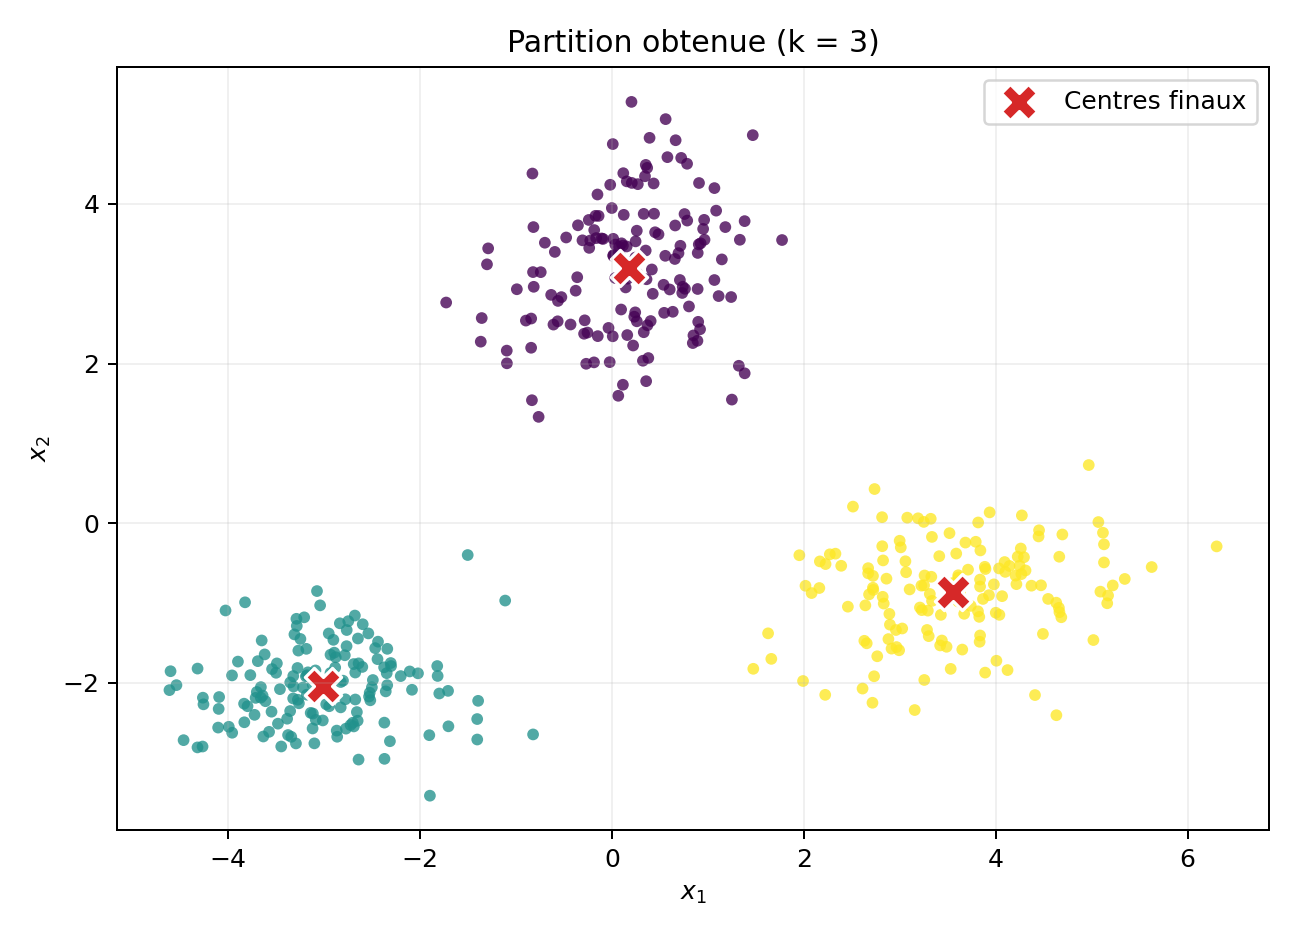
\includegraphics[width=.82\textwidth]{../figures/clusters.png}
 \caption{Classes découvertes et centres de gravité finaux.}
 \label{fig:clusters}
\end{figure}
Les trois groupes de la figure~\ref{fig:clusters} sont nettement séparés. Les
centres calculés sont proches des moyennes génératrices :
\[
 (0{,}183;3{,}203),\quad(-3{,}014;-2{,}035),\quad(3{,}554;-0{,}862).
\]
L'ordre des classes n'a pas de signification : une permutation des indices
décrit la même partition.

\subsection{Convergence}
\begin{figure}[H]
 \centering
 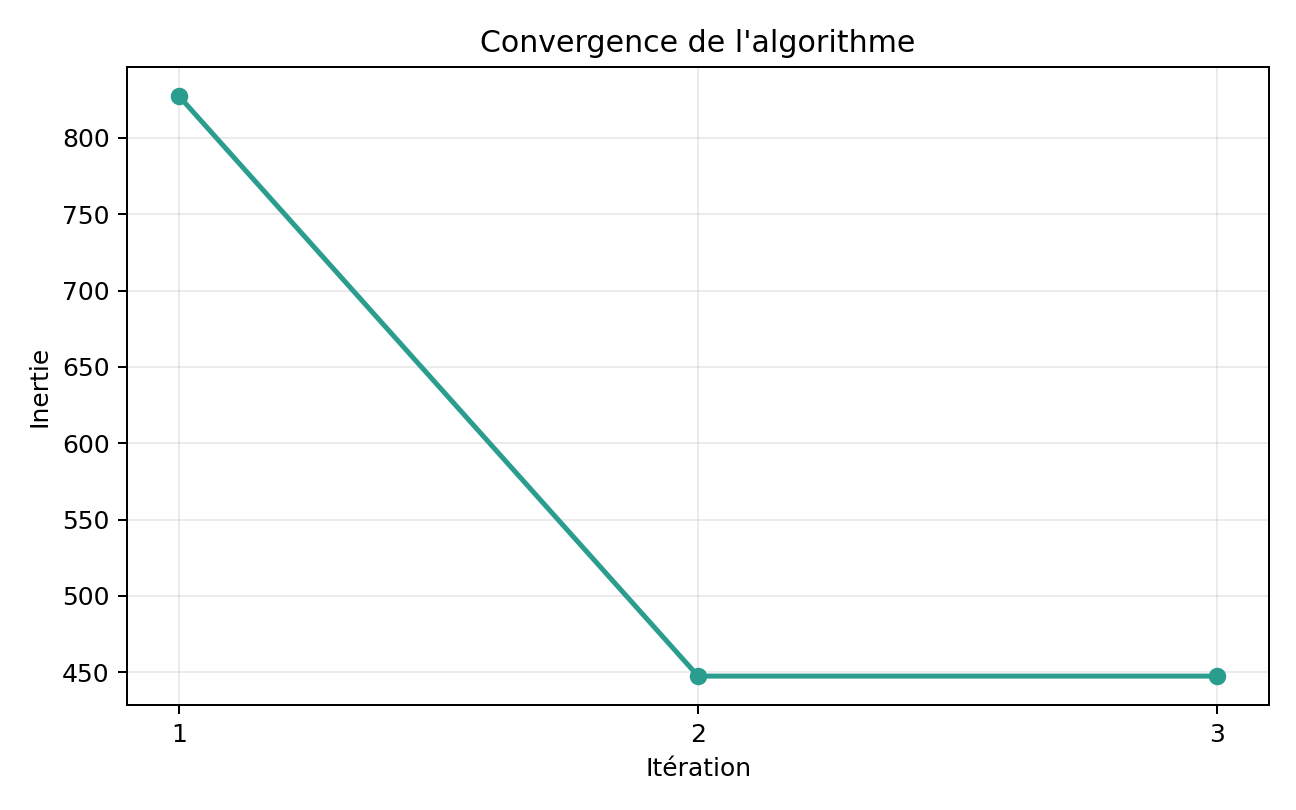
\includegraphics[width=.82\textwidth]{../figures/convergence.png}
 \caption{Évolution de l'inertie de la meilleure exécution.}
\end{figure}
La meilleure exécution atteint une inertie de $447{,}520831$ en deux
itérations. La décroissance puis la stabilisation observées sont conformes au
principe d'optimisation alternée.

\subsection{Choix du nombre de classes}
\begin{figure}[H]
 \centering
 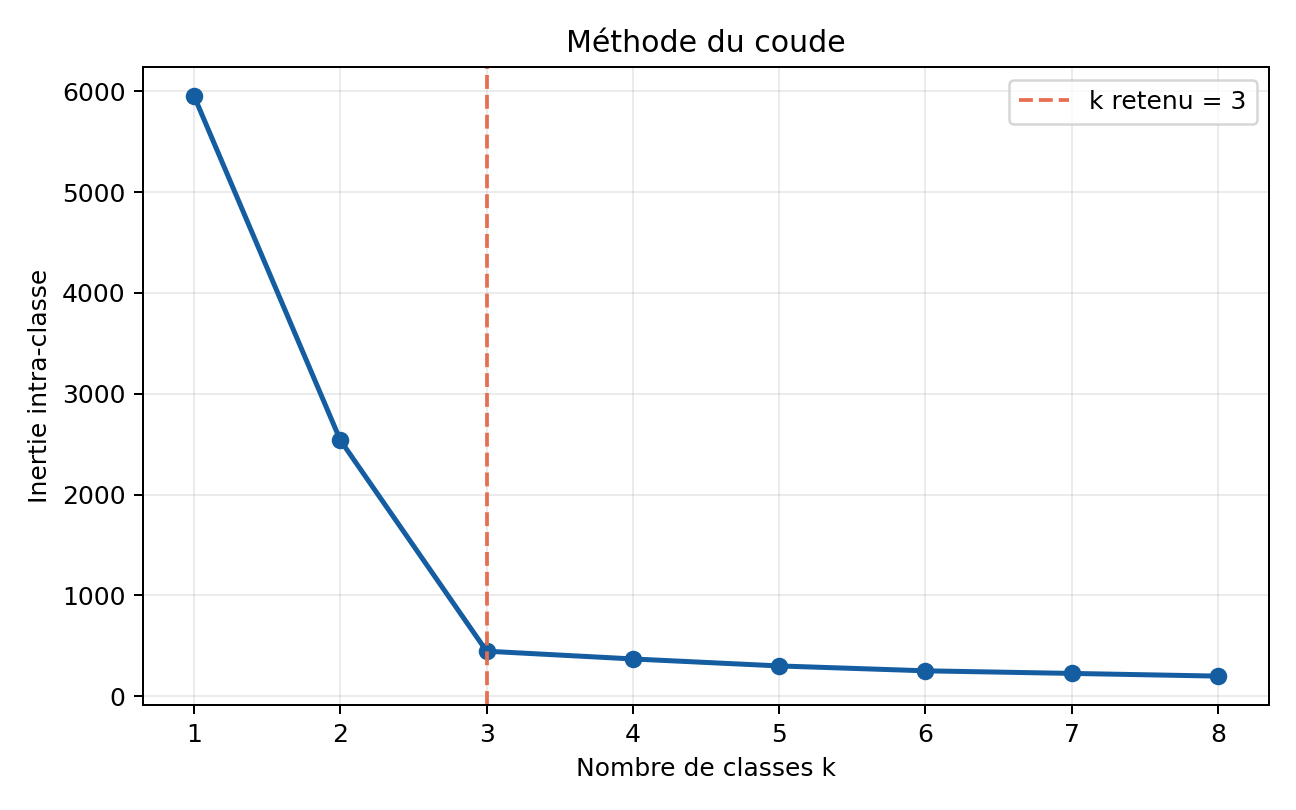
\includegraphics[width=.82\textwidth]{../figures/coude.png}
 \caption{Inertie en fonction du nombre de classes.}
\end{figure}
Le passage de $k=2$ ($2538{,}877$) à $k=3$ ($447{,}521$) apporte un gain majeur.
Après $k=3$, les diminutions deviennent beaucoup plus progressives. Le coude
confirme donc le choix de trois classes pour ce jeu de données.

\subsection{Validation comparative}
La comparaison n'intervient qu'après l'exécution du code personnel. Avec les
mêmes données, l'implémentation de référence décrite dans la documentation de
scikit-learn~\cite{sklearn2026} obtient elle aussi une inertie de
$447{,}520831$. L'indice de Rand ajusté (ARI) entre les deux partitions vaut
$1{,}000$, de même que l'ARI entre notre partition et les classes génératrices.
Cette égalité montre, pour l'expérience considérée, que les partitions sont
identiques à une permutation des étiquettes près.

\begin{table}[H]
\centering
\caption{Synthèse quantitative de l'expérience.}
\begin{tabular}{lr}
\toprule
Indicateur & Valeur\\
\midrule
Nombre d'observations & 450\\
Nombre de variables & 2\\
Nombre de classes & 3\\
Itérations de la meilleure exécution & 2\\
Inertie finale & 447,520831\\
ARI avec scikit-learn & 1,000000\\
ARI avec les classes génératrices & 1,000000\\
\bottomrule
\end{tabular}
\end{table}

\section{Limites et pistes d'amélioration}
L'algorithme exige que $k$ soit fixé à l'avance et reste sensible à
l'initialisation, malgré les redémarrages. La distance euclidienne le rend plus
adapté aux classes compactes et approximativement sphériques ; il décrit mal
les formes non convexes. Les variables de grande échelle peuvent dominer les
distances, d'où la nécessité de standardiser les données réelles. Enfin, les
valeurs aberrantes déplacent les moyennes.

Des extensions possibles comprennent l'initialisation $k$-means++
\cite{arthur2007}, la standardisation automatique, l'indice de silhouette pour
guider le choix de $k$, le traitement par mini-lots pour de grands volumes et
la comparaison avec DBSCAN ou un clustering hiérarchique.

\section{Reproductibilité et dépôt GitHub}
Le projet contient le code, les tests, les données, les figures et les sources
LaTeX. Après téléchargement, l'expérience s'exécute par :
\begin{lstlisting}[language=bash,numbers=none]
pip install -r requirements.txt
python experiments/experimentation.py
pytest -q
\end{lstlisting}
Le dépôt peut être publié à l'adresse suivante, à compléter après sa création :
\begin{center}
\url{https://github.com/VOTRE-COMPTE/nuees-dynamiques-from-scratch}
\end{center}
Le lien ne peut pas être rendu définitif avant la création effective du dépôt
sur le compte GitHub de l'étudiant.

\section{Conclusion}
Ce travail a construit l'algorithme des nuées dynamiques depuis ses opérations
élémentaires. La classe développée calcule manuellement les distances, alterne
affectation et mise à jour des centres, mesure l'inertie, traite les classes
vides, conserve l'historique de convergence et prédit la classe de nouveaux
points. Sur un jeu reproductible de 450 observations, elle retrouve parfaitement
les trois groupes générateurs et concorde avec la référence externe. Cette
réalisation met ainsi en évidence à la fois la simplicité, l'efficacité et les
limites de la méthode.

\bibliographystyle{plain}
\bibliography{references}
\end{document}
